\newpage
\section{Fazit}

In diesem Projekt haben wir ein neuronales Netz zur Detektion von horizontalen und oder vertikalen Balken entwickelt. Das neuronale Netz besteht dabei aus zwei Neuronen Schichten. Die Anzahl der benötigten Neuronen hängt dabei von der Anzahl der Merkmale ab. Die Anzahl der Neuronen in der ersten Ebene wächst Linear mit der Anzahl der Merkmale. Die erste Neuronen Ebene fasst dabei alle Pixel zu den jeweiligen Merkmalen zusammen. Jedes Pixel wird dabei über die Gewichts-Matrix bewertet. In der zweiten Neuronen Ebene findet eine Verfeinerung des Ergebnisses statt. Erst die zweite Neuronen Ebene wertet die Informationen aus den Merkmalen aus.

Entwickelt haben wir verschiedene Möglichkeiten von Gewichts-Matrizen. Untersucht haben wir am Ende die zwei erfolgversprechendsten Gewichts-Matrizen 'AddMul' und 'Special'. 'AddMul' hatte dabei die maximale Möglichkeit Parameter einzustellen. Dies ist bei der Special-Gewichtsmatrix nicht möglich. Vergleicht man beide Typen von Gewichts-Matrizen fällt kaum ein Unterschied im Ergebnis auf. Aus diesem Grund ist für uns die AddMul-Gewichts-Matrix besser geeignet, weil sie einfacher aufgebaut und variabler ist. Bei der Special-Gewichts-Matrix konnte sich ein Vorteil der erhöhten Randbereiche nicht bestätigen. Durch die Erhöhung haben sich lediglich die Schwellen der Detektion verändert.

Um die richtige Konfiguration der verschiedenen Parameter zu finden, haben wir länger gebraucht als erwartet. Es hat sich teilweise als sehr schwierig erwiesen vernünftige Werte zu finden. Die Ergebnisse hängen sehr stark davon ab, wie viel Rauschen man in den Bildern hat. Erste Einstellungen des neuronalen Netzes haben in komplett verrauschten Bildern ein Kreuz detektiert. Durch sukzessive Anpassung der Schwellen haben wir diesen Problem in den Griff bekommen. 

Ein weiteres Problem war es, die Merkmale der ersten Neuronen Ebene in zwei Gruppen zu unterteilen und damit separierbar zu machen. Jede Gruppe soll dabei möglichst zusammenhängend sein. Für das bessere Verständnis siehe Abbildung \ref{mGrup}. In diesem Fall muss die Flanke der Sigmoid-Funktion zwischen den beiden Gruppen liegen. Die Verschiebung der Sigmoid-Funktion wird über den jeweiligen Bias-Parameter erreicht. Mit dem Threshold-Parameter wird die Schwelle festgelegt, ab wann ein aktives Merkmal detektiert werden soll. Werden die Parameter 'pixelCnt', 'featureCnt', 'lowerBound', 'upperBound' oder 'slope' geändert, dann müssen auch die Parameter 'bias', 'threshold' und 'domainOfDefinition' neu eingestellt werden.

\begin{figure}[hbt]
	\centering
	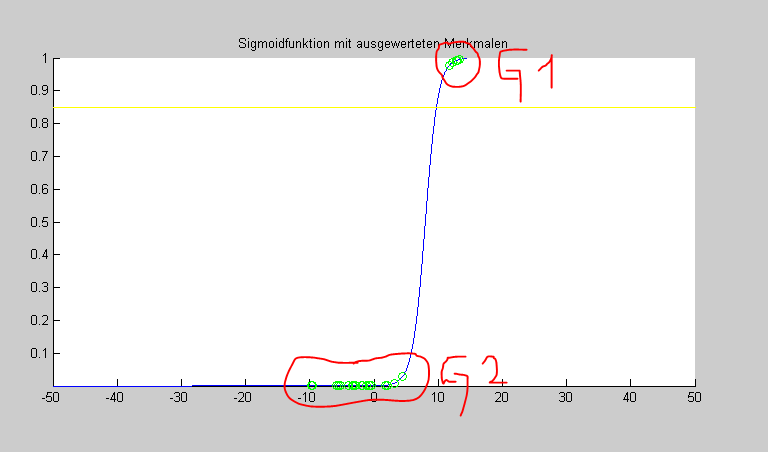
\includegraphics[trim=20 25 40 25, clip, width=0.9\linewidth]{./Bilder/Auswertung/MerkmalGruppen}
	\caption{Merkmale-Gruppen}
	\label{mGrup}
\end{figure}

Im Gegensatz zur ersten Ebene sind die richtigen Einstellungen für die zweite Ebene deutlich leichter zu finden, weil mal statt einer Sigmoid-Funktion drei Sigmoid-Funktionen zum Einstellen hat. Zur Erinnerung die zweite Neuronen Ebene erhält von der ersten Neuronen Ebene nicht die Werte der Sigmoid-Funktion, sondern die addierten Pixel-Gewichte ohne weitere Verarbeitung. Bei der zweiten Ebene können die Einstellungen für die Detektion des 'H-Balken', 'V-Balken' und des 'Fehlers' unabhängig voneinander eingestellt werden.

Mit dieser Arbeit haben wir einen Meilenstein gelegt, um ein Neuronales Netz in Hardware zu implementieren. Wir haben Erfahrungen gesammelt, wie ein selbst lernendes neuronales Netz die Gewichte findet und wie es aufgebaut sein muss, um vernünftige Ergebnisse zu liefern. Im Weiteren werden wir uns damit befassen unsere Ergebnisse in Hardware zu implementieren und weitere Funktionalitäten, wie zum Beispiel das selbstständige Lernen, zu ermöglichen.
